\documentclass[a4paper, 11pt, oneside]{article}

\usepackage[utf8]{inputenc}
\usepackage[T1]{fontenc}
\usepackage[french]{babel}
\usepackage{array}
\usepackage{shortvrb}
\usepackage{listings}
\usepackage[fleqn]{amsmath}
\frenchbsetup{StandardLists=true} % à inclure si on utilise \usepackage[french]{babel}
\usepackage{amsfonts}
\usepackage{fullpage}
\usepackage{enumerate}
\usepackage{graphicx}             % import, scale, and rotate graphics
\usepackage{subfigure}            % group figures
\usepackage{enumitem}
\usepackage{amssymb}
\usepackage{alltt}
\usepackage{url}
\usepackage{indentfirst}
\usepackage{eurosym}
\usepackage{listings}
\usepackage{color}
\usepackage[table,xcdraw,dvipsnames]{xcolor}
\usepackage{wrapfig}
\usepackage{minitoc}
\usepackage{clrscode3e}



% Change le nom par défaut des listing
\renewcommand{\lstlistingname}{Extrait de Code}

% Change la police des titres pour convenir à votre seul lecteur
\usepackage{sectsty}
\allsectionsfont{\sffamily\mdseries\upshape} 
% Idem pour la table des matière.
\usepackage[nottoc,notlof,notlot]{tocbibind} 
\usepackage[titles,subfigure]{tocloft} 
\renewcommand{\cftsecfont}{\rmfamily\mdseries\upshape}
\renewcommand{\cftsecpagefont}{\rmfamily\mdseries\upshape} 

\definecolor{mygray}{rgb}{0.5,0.5,0.5}
\newcommand{\coms}[1]{\textcolor{MidnightBlue}{#1}}

\lstset{
    language=C, % Utilisation du langage C
    commentstyle={\color{MidnightBlue}}, % Couleur des commentaires
    frame=single, % Entoure le code d'un joli cadre
    rulecolor=\color{black}, % Couleur de la ligne qui forme le cadre
    stringstyle=\color{RawSienna}, % Couleur des chaines de caractères
    numbers=left, % Ajoute une numérotation des lignes à gauche
    numbersep=5pt, % Distance entre les numérots de lignes et le code
    numberstyle=\tiny\color{mygray}, % Couleur des numéros de lignes
    basicstyle=\tt\footnotesize, 
    tabsize=3, % Largeur des tabulations par défaut
    keywordstyle=\tt\bf\footnotesize\color{Sepia}, % Style des mots-clés
    extendedchars=true, 
    captionpos=b, % sets the caption-position to bottom
    texcl=true, % Commentaires sur une ligne interprétés en Latex
    showstringspaces=false, % Ne montre pas les espace dans les chaines de caractères
    escapeinside={(>}{<)}, % Permet de mettre du latex entre des <( et )>.
    inputencoding=utf8,
    literate=
  {á}{{\'a}}1 {é}{{\'e}}1 {í}{{\'i}}1 {ó}{{\'o}}1 {ú}{{\'u}}1
  {Á}{{\'A}}1 {É}{{\'E}}1 {Í}{{\'I}}1 {Ó}{{\'O}}1 {Ú}{{\'U}}1
  {à}{{\`a}}1 {è}{{\`e}}1 {ì}{{\`i}}1 {ò}{{\`o}}1 {ù}{{\`u}}1
  {À}{{\`A}}1 {È}{{\`E}}1 {Ì}{{\`I}}1 {Ò}{{\`O}}1 {Ù}{{\`U}}1
  {ä}{{\"a}}1 {ë}{{\"e}}1 {ï}{{\"i}}1 {ö}{{\"o}}1 {ü}{{\"u}}1
  {Ä}{{\"A}}1 {Ë}{{\"E}}1 {Ï}{{\"I}}1 {Ö}{{\"O}}1 {Ü}{{\"U}}1
  {â}{{\^a}}1 {ê}{{\^e}}1 {î}{{\^i}}1 {ô}{{\^o}}1 {û}{{\^u}}1
  {Â}{{\^A}}1 {Ê}{{\^E}}1 {Î}{{\^I}}1 {Ô}{{\^O}}1 {Û}{{\^U}}1
  {œ}{{\oe}}1 {Œ}{{\OE}}1 {æ}{{\ae}}1 {Æ}{{\AE}}1 {ß}{{\ss}}1
  {ű}{{\H{u}}}1 {Ű}{{\H{U}}}1 {ő}{{\H{o}}}1 {Ő}{{\H{O}}}1
  {ç}{{\c c}}1 {Ç}{{\c C}}1 {ø}{{\o}}1 {å}{{\r a}}1 {Å}{{\r A}}1
  {€}{{\euro}}1 {£}{{\pounds}}1 {«}{{\guillemotleft}}1
  {»}{{\guillemotright}}1 {ñ}{{\~n}}1 {Ñ}{{\~N}}1 {¿}{{?`}}1
}
\newcommand{\tablemat}{~}

%%%%%%%%%%%%%%%%% TITRE %%%%%%%%%%%%%%%%
% Complétez et décommentez les définitions de macros suivantes :
 \newcommand{\intitule}{Projet 1: Algorithme de tri}
 \newcommand{\PrenomUN}{Julien}
 \newcommand{\NomUN}{Gustin}
 \newcommand{\PrenomDEUX}{Mathias}
 \newcommand{\NomDEUX}{Carlisi}
 %Décommentez ceci si vous voulez une table des matières :
 \renewcommand{\tablemat}{\tableofcontents}

%%%%%%%% ZONE PROTÉGÉE : MODIFIEZ UNE DES DIX PROCHAINES %%%%%%%%
%%%%%%%%            LIGNES POUR PERDRE 2 PTS.            %%%%%%%%
\title{INFO2050: \intitule}
\author{\PrenomUN~\textsc{\NomUN}, \PrenomDEUX~\textsc{\NomDEUX}}
\date{}
\begin{document}
\maketitle
\newpage
%%%%%%%%%%%%%%%%%%%% FIN DE LA ZONE PROTÉGÉE %%%%%%%%%%%%%%%%%%%%

%%%%%%%%%%%%%%%% RAPPORT %%%%%%%%%%%%%%%
% Écrivez votre rapport ci-dessous.

	\section{Analyse théorique}
	\subsection{Invariant}
	\begin{itemize}[label=$\square$]

\item

	\noindent $\{P\} \gets$ "$A$ est un tableau d'entiers de taille $\attrib{A}{length}"$\\
	  $\{Q\} \gets$ "Le tableau $A$ est trié"\\ 
	$\{I\} \gets$ "Le sous tableau 
$A[1..i]$ contient les $i$ premiers éléments de $A$ triés, le sous tableau \indent \indent $A[j..A.length]$ est la partie du tableau de $A$ qui n'est pas encore triée"

\item $\{P\} i = 1$ $\&\&$ $j = 2 \{I\}$
\\ $\{I\}$  $\exists i,j,$ $1 \leq i < j \leq \attrib{A}{length},$  $A[1..i],$ $\forall k,$ $1 \leq k < i, A[k] \leq A[k+1]$ \\
\indent Fonction de terminaison : $f \gets \attrib{A}{length}-j +1$
\\ $\{Q\} = \forall k,$ $1 \leq k < \attrib{A}{length},$ $A[k] \leq A[k+1]$ $\&\&$ $j=\attrib{A}{length}+1$

\end{itemize}

	\subsection{PseudoCode}
	\label{PseudoCode}
	
	\begin{codebox}
\Procname{$\proc{New-Sort}(A)$}
\li $i \gets 1$

\li \For $j \gets 2$ \To $\attrib{A}{length}$
\Do

\li \While $A[j] \leq A[j+1]$ and $j < \attrib{A}{length}$
\li \Do
$j \gets j + 1$
\End
\li $\proc{Merge}(A, 1, i, j)$

\li $i \gets j$
\End
\end{codebox}

\subsection{Complexité}
La complexité en temps, dans le meilleur des cas, est $\Theta(n)$ ( si le tableau est pré-trié par ordre croissant ) et dans le pire des cas $\Theta(n^{2})$ ( si le tableau est pré-trié dans un ordre décroissant ) , où 'n' est la taille du tableau ( array ).

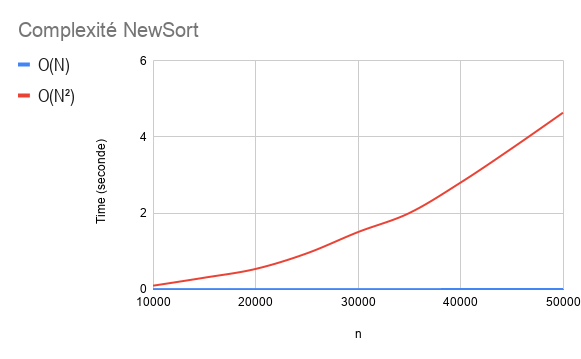
\includegraphics[scale=0.5]{graphique.png} \\
( Graphique testé avec des valeurs réelles ) %l'image est réduite de moitié


\subsection{Stabilité ?}
Le tri est stable parce que, grâce aux $A[j]\leq A[j+1]$, les valeurs égales n'interchangent pas de place, vu que \textit{Merge} est lui aussi stable NewSort ne peut etre que stable, ainsi le tri gagne en rapidité.
	\begin{codebox}

\li \While $A[j] \leq A[j+1]$ and $j < \attrib{A}{length}$
$\longrightarrow$ voir PseudoCode~\ref{PseudoCode}
\End
\end{codebox} 
\newpage
\subsection{Complexité au pire des cas}
\newpage

\section{Analyse expérimentale}
\subsection{Temps d'exécution sur des tableaux aléatoires}

\begin{table}[htb]
\begin{tabular}{cccccc}
\hline

n   & InsertionSort & QuickSort & HeapSort & MergeSort & NewSort \\ \hline
$10^{1}$ & 0,000015      & 0,000005  & 0,000006         & 0,000009          & 0,000005        \\
$10^{2}$ & 0,000052      & 0,000035  & 0,000061         & 0,000054          & 0,000090        \\
$10^{3}$ & 0,001055      & 0,000225  & 0,000959         & 0,000297          & 0,001841        \\
$10^{4}$ & 0,060314      & 0,003429  & 0,003847         & 0,002229          & 0,112815        \\
$10^{5}$ & 7,216459      & 0.036962  & 0,032527         & 0,017463           & 10,771157        \\
$10^{6}$ & 768,522644    & 2.639571  & 0,353273         & 0,179450          & 1429,154037
        
\end{tabular}
\end{table}

L'\textbf{InsertionSort} et le \textbf{NewSort} sont les tris les plus lents des cinq, en effet avec leurs complexités moyennes de $\Theta(n^{2})$, ces tris prennent un temps quadratique pour un tableau de taille 'n', cette complexité "élevée" découle du fait que, contrairement aux QuickSort, MergeSort ou HeapSort, ces tris requièrent (pour l'\textbf{InsertionSort}) de parcourir le tableau plusieurs fois pour insérer une valeur à sa bonne place et pour le \textbf{MergeSort}, de trié deux sous tableaux dont le premier commence de la première case jusqu'à la dernière précédemment triée, et le deuxième, de la case qui suit le premier sous tableau jusqu'à la dernière case où la suivante  n'est pas triée par ordre croissant, et ainsi la fusion de ces deux sous-tableaux pré-triés crée un tableau trié.
 Parcourir plusieurs fois le tableau mène à une complexité de $\Theta(n^{2})$.
\\
\\
L'algorithme qui suit est de type "diviser pour régner" ( découper le problème initial en sous problèmes, résoudre ceux ci permettent de résoudre le problème initial ), sa complexité moyenne est $\Theta(n$ $log$ $n$) cependant, au pire des cas, est quadratique ce qui est la cause de sa "lenteur" comparé aux HeapSort et MergeSort, le \textbf{QuickSort} procède par une méthode qui s'appelle "partition" et qui consiste à choisir un pivot que nous plaçons à la fin du sous tableau. Les éléments inférieurs à celui ci sont insérés au début de ce sous tableau, ensuite ce pivot est placé à la fin des éléments déplacés, cette méthode permet de trier le tableau rapidement, cependant, si le tableau est déjà trié en entrée, ce tri n'est pas vraiment efficace.\\ 

Les deux prochains algorithmes, \textbf{HeapSort} et \textbf{MergeSort} sont tout deux extrêmement rapide avec une complexité que ce soit dans le pire ou meilleur des cas de $\Theta(n$ $log$ $n$) soit de complexité asymptotiquement optimale, le \textbf{MergeSort} est de type " diviser pour régner", cet algorithme fonctionne par le principe que à partir de deux tableaux triés nous pouvons formé un tableau triés ainsi par récursivité nous créons des sous-tableaux de plus en plus petit jusqu'à ce que le tableau ne contienne qu'un seul élément et par la remonté récursive nous fusionnons ces tableaux qui deviennent de plus en plus grands à chaque remonté jusqu'à ce que le tableau soit complètement trié.\\ Le \textbf{HeapSort} fonctionne par arbre binaire.
Ce qui crée la légère différence en temps entre ces deux tris est la stabilité en effet le HeapSort ne préserve pas nécessairement l’ordre des éléments à valeurs identique contrairement au MergeSort qui gagne ainsi en rapidité.

\begin{table}[htb]
\begin{tabular}{cccccc}
\hline

Cas   & InsertionSort & QuickSort & HeapSort & MergeSort & NewSort \\ \hline
Meilleur & $\Theta(n)$      & $\Theta(n$ $log$ $n)$   & $\Theta(n$ $log$ $n)$        & $\Theta(n$ $log$ $n)$          & $\Theta(n)$        \\
Pire & $\Theta(n^{2})$     & $\Theta(n^{2})$  & $\Theta(n$ $log$ $n)$         & $\Theta(n$ $log$ $n)$ & $\Theta(n^{2})$       \\
Moyen & $\Theta(n^{2})$      & $\Theta(n$ $log$ $n)$  & $\Theta(n$ $log$ $n)$         & $\Theta(n$ $log$ $n)$         & $\Theta(n^{2})$        \\
Stable & Oui      & Non  & Non         & Oui          & Oui        \\
  
\end{tabular}
\end{table}

\end{document}